%%%%%%%%%%%%%%%%%%%%%%%%%%%%%%%%%%%%%%%%%%%%%%%%%%%%%%%%%%%%%%%%%%%%%%%%%%%%%%%%%%%%%%%%%%%%%%%%%%%%%%%%%%%%%%%%%%%%%%%%%%%%%
\section{Introduction}\label{sec:introduction}

%%%%%%%%%%%%%%%%%%%%%%%%%%%%%%%%%%%%%%%%%%%%%%%%%%%%%%%%%%%%%%%%%%%%%%%%%%%%%%%%%%%%%%%%%%%%%%%%%%%%%%%%%%%%%%%%%%%%%%%%%%%%%
\section{Literature Review}\label{sec:literature_review}

  \subsection{Fire Detection with Computer Vision}

  \subsection{Existing Fire Image Datasets}

%%%%%%%%%%%%%%%%%%%%%%%%%%%%%%%%%%%%%%%%%%%%%%%%%%%%%%%%%%%%%%%%%%%%%%%%%%%%%%%%%%%%%%%%%%%%%%%%%%%%%%%%%%%%%%%%%%%%%%%%%%%%%
\section{Hardware Design}\label{sec:hardware}
  
  \subsection{Overview}
  Although not crucial

  \subsection{Drone}

  \subsubsection{Rationale for building custom UAV}

  The primary design consideration in building this system was enabling hardware-accelerated neural network inference on edge.
  There are few notable instances of using AI hardware accelerators in existing commercial drones.
  For example, DJI Mavic and DJI Phantom drones use Intel VPU chips for vision-based obstacle avoidance. 
  Another example is Skydio 2, which utilizes Nvidia Tegra TX2 processor for vision-based navigation and obstacle avoidance.

  Unfortunately, at the time of writing this thesis, there are no readily available low-cost drones that would provide developers and researchers
  programmatic access to the AI chip. 
  
  In the sections \ref{sec:sensors} I cover the design of the UAV platform, as well as the Camera-Compute Payload, enabling the system's perception.

  \subsubsection{Sensors}\label{sec:sensors}


  \paragraph{RTK GNSS}

  % TODO: image of stddev of two sensors

  \subsection{Payload}
  Talk about the payload 

%%%%%%%%%%%%%%%%%%%%%%%%%%%%%%%%%%%%%%%%%%%%%%%%%%%%%%%%%%%%%%%%%%%%%%%%%%%%%%%%%%%%%%%%%%%%%%%%%%%%%%%%%%%%%%%%%%%%%%%%%%%%%

\section{Fire Incident Aerial Image Dataset}\label{sec:dataset}

  \subsection{The rationale for creating a new datset}

  \subsection{Acquisiton}
  \begin{figure}
    \centering
    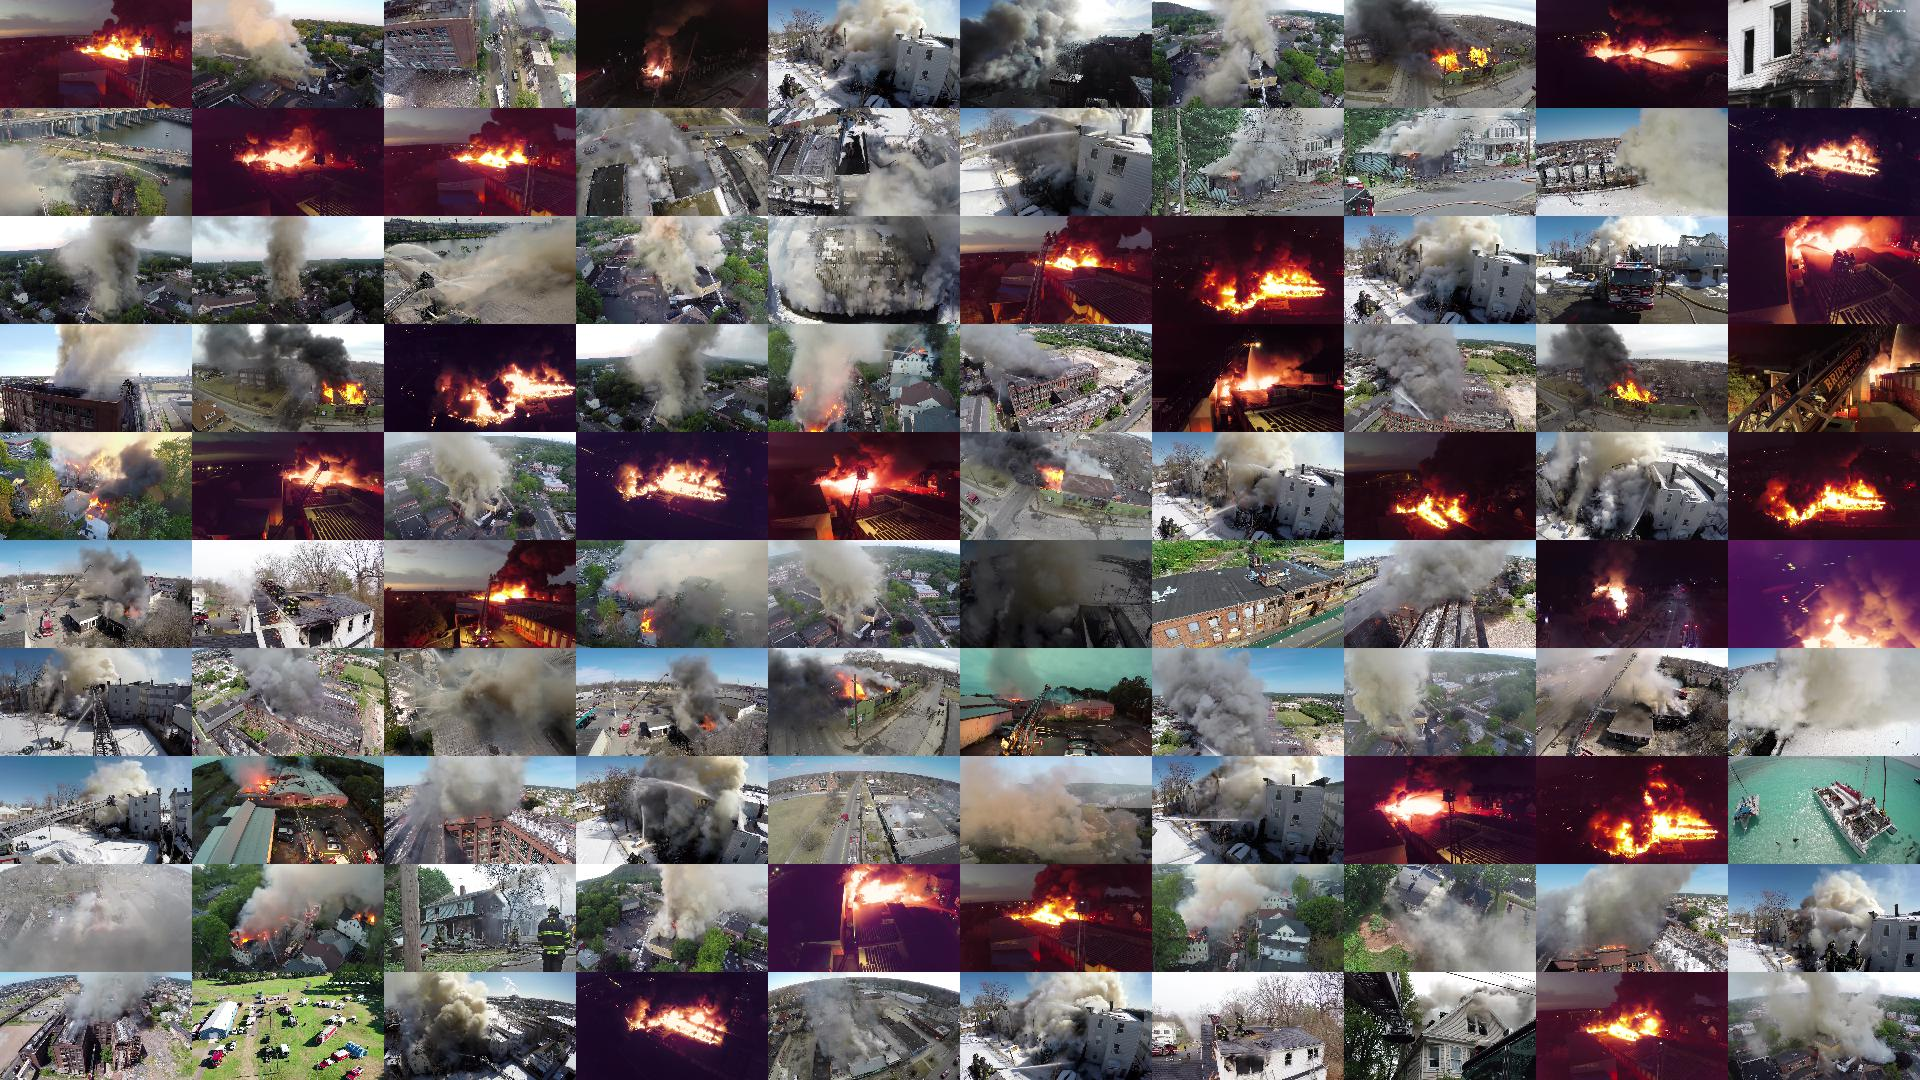
\includegraphics[width=\linewidth]{figures/lowres_100tiles.jpg}
    \caption{100 samples from the dataset}
  \end{figure}

  \subsection{Annotations}
  % TODO

\section{Fire Detection Model}\label{sec:detection}

  \subsection{Model}

  \subsection{Training}
    
  \subsection{Evaluation}

  \subsection{Evaluation - GradCAM}

\section{Auxilary Vision Systems}\label{sec:other}

  \subsection{Person Detection}

\section{End-to-end System Testing}

  \section{Environment Simulation}

%%%%%%%%%%%%%%%%%%%%%%%%%%%%%%%%%%%%%%%%%%%%%%%%%%%%%%%%%%%%%%%%%%%%%%%%%%%%%%%%%%%%%%%%%%%%%%%%%%%%%%%%%%%%%%%%%%%%%%%%%%%%%%
\section{Future Work}\label{sec:future_work}

  \subsection{RL control}

  \subsection{Field Testing}

%%%%%%%%%%%%%%%%%%%%%%%%%%%%%%%%%%%%%%%%%%%%%%%%%%%%%%%%%%%%%%%%%%%%%%%%%%%%%%%%%%%%%%%%%%%%%%%%%%%%%%%%%%%%%%%%%%%%%%%%%%%%%%
\section{Conclusions}\label{sec:conclusions}


